	\documentclass[fleqn, 12pt]{article}
	\usepackage[latin1]{inputenc}
	\usepackage[ngerman]{babel}
	\usepackage[a4paper,text={155mm,220mm},centering,headsep=10mm,footskip=15mm]{geometry}
	\usepackage{graphicx}
	\usepackage{amssymb}
	\usepackage{graphicx}
	\usepackage{multirow}
	\usepackage{multicol}
	\usepackage{pst-plot}
	\usepackage{float}
	\usepackage{pdfpages}
	\usepackage{todonotes}
	\title{}
	\date{}
	\author{}
	\usepackage{array}
	\usepackage{amsmath}
	\usepackage{fancyhdr}
	\usepackage{enumitem} 
	\parindent0pt
	\usepackage[format=plain,
      justification=RaggedRight,
      singlelinecheck=false]
     {caption}

	
	% Listings
	\usepackage{listings}
	\renewcommand{\lstlistlistingname}{Liste der Quellcode Ausschnitte}
	\renewcommand{\lstlistingname}{Quellcode Ausschnitt}
		\definecolor{lsgreen}{rgb}{0,.5,0}
		\definecolor{lsred}{rgb}{.7,0,0}
		\definecolor{lsorange}{rgb}{.9,.5,0}
		\definecolor{lsgray}{rgb}{.5,.5,.5}
		\lstset{
			frame=tb,
			aboveskip=10mm,
			belowskip=10mm,
			showstringspaces=false,
			columns=flexible,
			captionpos=b,
			basicstyle={\normalsize\ttfamily},
			numbers=left,
			numberstyle=\tiny\color{lsgray},
			keywordstyle=\color{blue},
			commentstyle=\color{lsorange},
			stringstyle=\color{lsgreen},
			breaklines=true,
			breakatwhitespace=true,
			rulecolor=\color{lsgray},
			xleftmargin=7mm,
			tabsize=3
		}
	
	% Needed for proper display of links in bibliography
	\usepackage{url}	
	
	% Hyperref
	\usepackage[
	pdfauthor={Laura Anger, Timo \dots, Lukas Kolhagen},
	pdftitle={BVA Bewegungsanalyse},
	pdftoolbar=true,	
	colorlinks=true,
	linkcolor=blue,
	citecolor=blue,
	urlcolor=blue,
	linktocpage=true
	]{hyperref}
	\usepackage{bookmark}
	\bookmarksetup{
	numbered
	}
	\urlstyle{same}
	
	\pagestyle{fancy}
	\fancyhf{}
	\fancyhead[LO]{BVA}
	\fancyhead[CO]{Bewegungsanalyse in einer Videosequenz}
	\fancyhead[RO]{\thepage}
	\renewcommand{\headrulewidth}{0.5pt}
	\newcommand{\Absatzbox}[1]{\parbox[0pt][2em][c]{0cm}{}}
	
	% Itemize symbol
	\renewcommand{\labelitemi}{$\triangleright$}
	
	% Colors
	\definecolor{yellow}{rgb}{.95,.85,0}
	\definecolor{green}{rgb}{0,.8,0}
	\definecolor{blue}{rgb}{0,0,.8}
	\definecolor{red}{rgb}{.8,0,0}
	\definecolor{grey}{rgb}{.4,.4,.4}
	\definecolor{orange}{rgb}{.9,.5,0}
	
	% Macro for typesetting C++
	\newcommand{\CC}{C\nolinebreak\hspace{-.05em}\raisebox{.4ex}{\tiny\bf +}\nolinebreak\hspace{-.10em}\raisebox{.4ex}{\tiny\bf +}}
\def\CC{{C\nolinebreak[4]\hspace{-.05em}\raisebox{.4ex}{\tiny\bf ++}}}

\begin{document}
\thispagestyle{empty}
	%\sffamily
			\begin{center}
			
\includegraphics[width=.35\textwidth]{logo_TH}\\[20ex]
			{\Huge\textbf{Projektdokumentation}}\\[8ex]
			\rule{.8\textwidth}{.2pt}
			{\Large Bewegungsanalyse in einer Videosequenz\\[1ex] mit dem Ansatz des Papers
			von Aach und Kunz}\\
			\rule{.8\textwidth}{.2pt}\\[10ex]
			von\\[2ex]
			\begin{tabular}{ll}
			Laura Anger &(Matrikelnr. 11086356)\\ 
			Timo Breuer &(Matrikelnr. XXXXXXXX)\\ 
			Lukas Kolhagen &(Matrikelnr. 11084355)\\
			\end{tabular}\\[10ex]
			Durchgef�hrt im\\ \textbf{Master Medientechnologie}\\ im\\ 
			\textbf{Sommersemester 2016}\\			
			\end{center}
			\vfill
			\begin{flushleft}
			{\bf Betreuer:}\\
			Prof. Dr. Dietmar Kunz\\
			Institut f�r Medien- und Phototechnik
			\end{flushleft}
	\newpage
	\tableofcontents
	\newpage
	\section{Einleitung}\todo[inline]{Lukas}
	Diese Ausarbeitung ist Teil der Abschlussprojekt-Dokumentation im Modul "`Weiterf�hrende Themen der Bildverarbeitung"' im Master Medientechnologie an der Technischen Hochschule K�ln.
	
	Das Projekt besch�ftigte sich mit der Bewegungsanalyse einer Videosequenz mit dem Ansatz des Papers von Aach und Kunz\textsuperscript{\cite{aach1998bayesian}}. Es wurde bearbeitet von Laura Anger, Timo Breuer und Lukas Kolhagen.		
	\subsection{Ansatz im Paper von Aach und Kunz}
	\section{Verfahren}
		\subsection{Bewegungssch�tzung}\todo[inline]{Laura}
		\subsection{Programmablauf}\todo[inline]{Lukas}
		\subsection{Kostenfunktion}\todo[inline]{Alle}
			\subsubsection{Datenterm}\todo[inline]{Lukas}
			\subsubsection{�rtliche Koh�renz}\todo[inline]{Timo}
			\subsubsection{Zeitliche Koh�renz}\todo[inline]{Lukas}
		\subsection{Visualisierung}\todo[inline]{Laura}
	\section{Auswertung}\todo[inline]{Laura \& Timo}

\subsection{Testmaterial}\todo[inline]{Laura}
Das Verfahren wird an drei unterschiedlichen Bildsequenzen getestet, die im Folgenden Testmaterial 1-3 genannt werden und alle eine Aufl�sung von 256x2656 Pixeln haben. Bei Testmaterial 1 und Testmaterial 2 wurde ein Bild um bekannte Werte in x- und y-Richtung verschoben. Anzumerken ist auch, dass beide Testmaterialien identisch verschoben wurden. Bei Testmaterial 3 kann die Bewegung der zu sehenden Objekte lediglich gesch�tzt werden. Alle Testmaterialien wurden f�r diese Dokumentation aufgenommen bzw. erstellt.\vspace{0.6cm}

\begin{minipage}{0.5\textwidth}
\begin{figure}[H] 
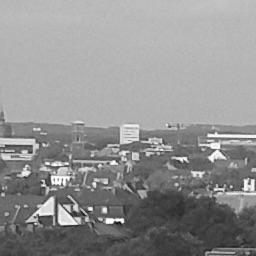
\includegraphics[scale=0.77]{Testmaterial1.jpg}
\caption{Standbild Testmaterial 1}
\end{figure}
\end{minipage}
\begin{minipage}{0.5\textwidth}
\textbf{Testmaterial 1}\\
Diese Bildsequenz besteht aus 150 Frames und wurde aus einem Bild der Stadt K�ln erzeugt.\\ 
Bei den ersten und letzten 50 Frames wird ein Ausschnitt des Bildes um jeweils 10 Pixel nach rechts bzw. unten verschoben. In den mittleren 50 Frames  wird der Bildinhalt um 10 Pixel nach rechts und 10 Pixel nach unten verschoben. 
\vspace{2.0cm}\\
\end{minipage}\vspace{0.7cm}

\begin{minipage}{0.5\textwidth}
\begin{figure}[H] 
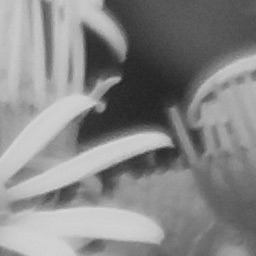
\includegraphics[scale=0.77]{Testmaterial2.jpg}
\caption{Standbild Testmaterial 2}
\end{figure}
\end{minipage}
\begin{minipage}{0.5\textwidth}
\textbf{Testmaterial 2}\\
Auf den 150 Frames, die diese Bildsequenz umfasst ist ein Blumenmotiv zu sehen, welches jeweils �ber 50 Frames in verschiedene Richtungen verschoben wird. Auf den ersten Frames erfolgt eine Verschiebung um 10 Pixel nach rechts. W�hrend die mittleren Frames um sowohl 10 Pixel nach rechts, als auch 10 Pixel nach unten verschoben wurden, wurde der Bildinhalt der verbleibenden Frames nur um 10 Pixel nach unten verschoben.
\vspace{1.0cm}\\
\end{minipage}\vspace{0.7cm}


\begin{minipage}{0.5\textwidth}
\begin{figure}[H] 
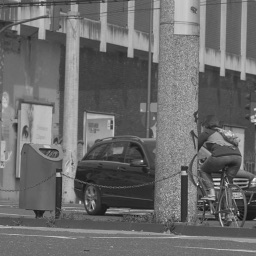
\includegraphics[scale=0.77]{Testmaterial3.jpg}
\caption{Standbild Testmaterial 3}
\end{figure}
\end{minipage}
\begin{minipage}{0.5\textwidth}
\textbf{Testmaterial 3}\\
Bei Testmaterial 3 handelt es sich um eine reale Videosequenz, die in K�ln Ehrenfeld aufgenommen wurde. Zu sehen sind ein Auto, dass sich von links nach rechts durch das Bild bewegt und eine Fahrradfahrerin, die das Bild genau entgegengesetzt durchf�hrt. Beide Objekte werden zeitweise durch eine S�ule verdeckt. Die Kamera ist starr, weshalb f�r den restlichen Bildinhalt keine Bewegung zu erkennen ist. 
\vspace{1.1cm}\\
\end{minipage}

		\subsection{Analyse der Kostenfunktion}\todo[inline]{Laura}
		\subsection{Einschwingverhalten}
			\subsubsection{Bewegungsvektorfelder}\todo[inline]{Timo}
			\subsubsection{Innerhalb eines Bildes}\todo[inline]{Laura}
		\subsection{Parameter der Regularisierungsterme}\todo[inline]{Timo}
	\section{Zusammenfassung}\todo[inline]{Lukas}
	\section{Arbeitsaufteilung der Dokumentation}
	\newpage
	\bibliographystyle{plain}
	\bibliography{ABV_Bewegungsanalyse_LaTeX}
\end{document}
		